\chapter{Objectifs de commande}
\minitoc
\label{chap:objectif}

\section{Contexte opérationnel}
Tout l'intérêt des drones est leurs capacités à se maintenir stabilisé sans intervention humaine. Ainsi, les opérateurs peuvent se concentrer sur la mission, sans devoir consacrer une grande attention au pilotage du drone. 

Les nombreux progrès dans les systèmes d'estimation état permettent de connaitre précisément l'orientation et la position des drones pour assurer la stabilisation, le guidage et la navigation. Les progrès sont lié à l'amélioration continue des capteurs, notamment des centrales inertielles (Inertial Measurement Units, IMU), \nomenclature[]{\(IMU\)}{Centrales inertielles (\textit{Inertial Measurement Units})} constitué d'un accéléromètre, d'un gyroscope et d'un magnétomètre. La Table \ref{tab:autopilote_ev} montre l'évolution des vitesses des microcontrôleurs (Microcontroller Unit, MCU) \nomenclature[]{\(MCU\)}{Microcontrôleurs (\textit{Microcontroller Unit})} embarqué sur les autopilotes et de la réduction du bruit des capteurs inertiel.
\begin{table}[ht]
    \centering
    \begin{tabular}{|c|c|c|c|c|c|}
        \hline
        Type & Date & MCU & Vitesse & Capteur  & Bruit RMS \\
        \hline \hline
        \href{https://wiki.paparazziuav.org/wiki/Apogee/v1.00}{Apogee}  & 2013 & STM32F4 & 168 MHz & MPU-9150 & \begin{tabular}{ccc} Gyro : 0.06 dps \\
        Accel: 4 mg  \end{tabular}  \\
        \hline
        \href{https://wiki.paparazziuav.org/wiki/Chimera/v1.00}{Chimera} & 2016 & STM32F7 & 216 MHz &  MPU-9250 & \begin{tabular}{ccc} Gyro : 0.1  dps \\
        Accel: 8 mg  \end{tabular}\\
        \hline
        \href{https://wiki.paparazziuav.org/wiki/Tawaki/v1.10}{Tawaki 1} &2019 &  STM32F7 & 216 MHz  & ICM-20600 & \begin{tabular}{ccc} Gyro : 0.04 dps \\
        Accel: 1 mg  \end{tabular}\\
        \hline
        \href{https://wiki.paparazziuav.org/wiki/Tawaki/v2.01}{Tawaki 2} &2023 &  STM32H7 & 480 MHz & ICM-42688-P & \begin{tabular}{ccc} Gyro : 0.028 dps \\
        Accel: 0.70 mg  \end{tabular} \\
        \hline
    \end{tabular}
    \caption{Évolution des autopilotes paparazzi sur dix ans.}
    \label{tab:autopilote_ev}
\end{table}

Sur une période de dix ans, nous pouvons observer que les microcontrôleurs ont doublé leurs vitesses d'exécution, que les fabricants ont divisé par deux le bruit moyen sur les gyroscopes et par quatre le bruit moyen des accéléromètres.
Ces évolutions continues permettent une amélioration de l'estimation du drone utilisé pour la stabilisation. Il en résulte une stabilité accrue et de nouvelle possibilité pour la commande des drones.


\section{Contexte de la thèse}
De nombreux travaux ont été mener sur les \textit{tailsitters}, avec l'objectif de couvrir l'intégralité du domaine de vol. 
Nous pouvons citer en exemple le \textit{tailsitter} à double rotor appelé « T-Wing » \cite{Stone2002PreliminaryDO, TWing2008}, un autre tail-sitter appelé « MavIon » \cite{oatao14575}, ou le « JLion » et le « KH-Lion » \cite{8003167}. Ces drones partagent une architecture similaire basée sur une aile supportant deux moteurs sur le bord d'attaque et soufflant deux élevons situés sur le bord de fuite. Cette architecture offre une plus grande robustesse que les \textit{tiltrotors}, qui nécessitent des pièces mobiles, ce qui les rend plus fragiles et un actionneur puissant pour faire tourner l'ensemble moteur-hélice.
La complexité inhérente à ces architectures nécessite un travail de modélisation en raison des nombreuses non-linéarités et couplages impliqués, en particulier en termes de modélisation des effets aérodynamiques. Dans ce contexte, l'interférence aérodynamique entre l'aile fixe et les rotors a été modélisée dans \cite{droandi_zanotti_gibertini_grassi_campanardi_2015, Simmons2022, aerospace5030079}, et les forces et moments d'hélice générés à des angles d'attaque élevés sont abordés dans \cite{Fernandez2023}. Cependant, ces modèles sont complexes et ne sont que partiellement utilisables pour la conception des commandes. 

Un autre point important est la représentation de l'attitude du drone. Il est possible de représenter son orientation par des angles d'Euler \cite{4177650, 5415267, 8003165}, ce qui permet une compréhension intuitive, mais une singularité apparaît dans certaines phases de vol. Compte tenu de la grande manœuvrabilité, il est préférable de représenter l'attitude par un quaternion unitaire, ce qui élimine toute singularité \cite{8027691}. De nombreuses publications modélisent les effets aérodynamiques en fonction de l'angle d'attaque et du dérapage générés par les hélices \cite{Escareno07, 8453301}. 
Il est possible de choisir un autre modèle pour les interactions aérodynamiques entre les moteurs, les ailes et les élevons, comme présenté dans \cite{lustosaHal-03035938}. La technique de modélisation présentée dans \cite{lustosaHal-03035938} permet de disposer d'un modèle global couvrant l'ensemble de l'enveloppe de vol, grâce à ce que l'on appelle l'approche théorique $\Phi$. Bien que l'approche théorique $\Phi$ ne permette pas de prédire la chute brutale de la force de portance avec un angle d'attaque (AoA) croissant (qui est causée par un flux d'air turbulent) \cite{tal2022global}, elle permet de représenter le drone avec suffisamment de précision pour capturer le comportement lors de manœuvres agressives. 


Ce dernier est constitué des phases de vol suivantes :
\begin{enumerate}
    \item Décollage vertical
    \item Transition entre le vol stationnaire et le vol d'avancement
    \item Vol d'avancement
    \item Transition entre le vol d'avancement et le vol stationnaire
    \item Atterrissage vertical
\end{enumerate}
Bien que l'on puisse observer une symétrie dans la phase \raisebox{.5pt}{\textcircled{\raisebox{-.9pt} {1}}} et \raisebox{.5pt}{\textcircled{\raisebox{-.9pt} {5}}}, qui correspondent au décollage et à l'atterrissage vertical, une différence fondamentale est observé. Lors du décollage, la vitesse du drone engendrera un flux d'aire sur l'aile orienté dans le même sens que le flux d'air généré par les hélices. Cependant, lors de l'atterrissage, le flux d'air va se trouver inversé, le drone doit descendre, ce qui engendre une vitesse opposée à la direction du flux d'air des hélices. Cette inversion génère une instabilité qui doit être compensé par le contrôleur.

Le vecteur $\overrightarrow{W}$ représente la perturbation de vent qui peut affecter le vol sur l'intégralité des cinq phases de vol. Toutefois, on observe que dans les phases décollage \raisebox{.5pt}{\textcircled{\raisebox{-.9pt} {1}}}, de transition \raisebox{.5pt}{\textcircled{\raisebox{-.9pt} {2}}} et \raisebox{.5pt}{\textcircled{\raisebox{-.9pt} {4}}} et d'atterrissage \raisebox{.5pt}{\textcircled{\raisebox{-.9pt} {5}}} le drone offre une grande surface verticale sujette au vent. Ainsi, il est nécessaire de traité l'impact du vent sur cette architecture.

\begin{figure}[ht!]
    \centering
        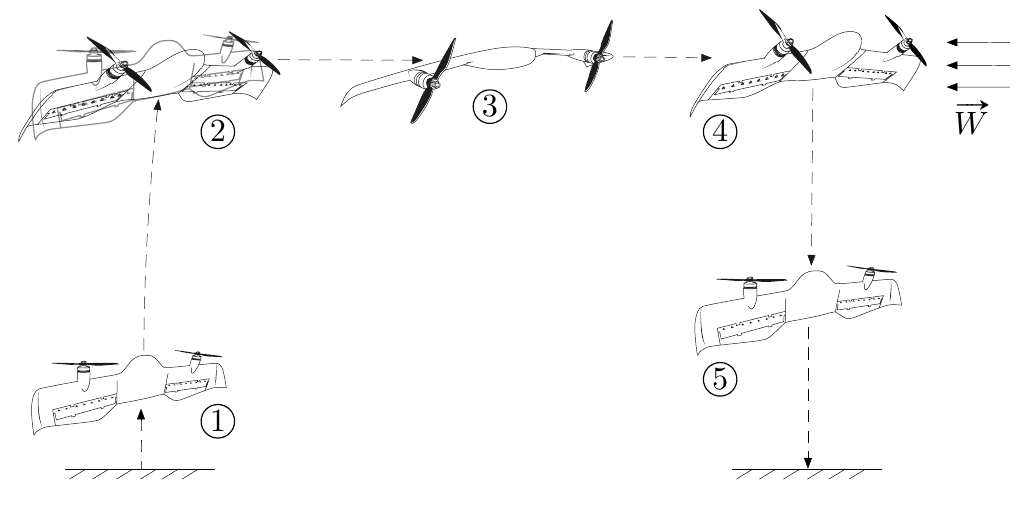
\includegraphics[width=0.8\columnwidth]{figures/darko_transition.png}
        \caption{Phase de vol d'un drone \textit{tailsitters}, DarkO.}
        \label{fig:darko_flight}
\end{figure}

Actuellement, nous pouvons mentionner deux types d'architecture de commande ayant fonctionné sur ce tailsitter. La première est basée sur une inversion incrémentale de la dynamique du drone (\textit{Incremental Non-linear Dynamic Inversion}, INDI) et la seconde est basée sur le technique sans modèle (\textit{Model free control}, MFC).




\todo{rejet de perturbation et metrique de maintient de position }


\section{Résumée}